% Chapter Template

\chapter{Results} % Main chapter title

\label{Chapter6} % Change X to a consecutive number; for referencing this chapter elsewhere, use \ref{ChapterX}

\lhead{Chapter 6. \emph{Results}} % Change X to a consecutive number; this is for the header on each page - perhaps a shortened title




\section{Results}

We trained our model on all available Mushaf recitations, reserving Mushaf 26.1 and 19.0 exclusively for testing. The evaluation results are summarized in Table \ref{tab:results}. The achieved Average Phoneme Error Rate (PER) of 0.16\% strongly supports our hypothesis that the Quran Phonetic Script is learnable using modern speech processing techniques.

We further tested the model on actual samples containing errors in \arb{مد}, \arb{غنة}, \arb{قلقلة}, and \arb{تفخيم}. Despite being trained only on error-free expert recitations, the model successfully detected these common pronunciation mistakes. While these preliminary results are promising, a more comprehensive evaluation on dedicated error-annotated datasets—such as \cite{khan2021tarteel}—is planned for future work.

We observe that the PER is well-balanced across nearly all phonetic and attribute levels, with the exception of the phoneme level itself. This is expected, as the phoneme level has a significantly larger vocabulary (44 symbols, including padding), increasing its complexity relative to the attribute levels.


\begin{table}[htbp]
\centering
\caption{Test results on Mushaf 26.1 and 19.0. The Average Phoneme Error Rate (PER) is \textbf{0.16\%}, confirming the learnability of the Quran Phonetic Script. The phoneme-level PER is higher (0.54\%) due to its larger vocabulary.}
\label{tab:results}\\
\vspace{3pt}
\label{tab:results}
\begin{tabular}{lc}
\hline
\textbf{Metric} & \textbf{Value} \\
\hline
loss & 0.01162 \\
per\_phonemes & 0.00543 \\
per\_hams\_or\_jahr & 0.00117 \\
per\_shidda\_or\_rakhawa & 0.00172 \\
per\_tafkheem\_or\_taqeeq & 0.00167 \\
per\_itbaq & 0.00092 \\
per\_safeer & 0.00132 \\
per\_qalqla & 0.00085 \\
per\_tikraar & 0.0009 \\
per\_tafashie & 0.0016 \\
per\_istitala & 0.0008 \\
per\_ghonna & 0.0013 \\
average\_per & \textbf{0.0016} \\
\hline
\end{tabular}
\end{table}


To evaluate real-world performance, we developed a demonstration application using Gradio\footnote{https://www.gradio.app/}. The interface allows users to record or upload their recitations and receive immediate phonetic and attribute-level feedback.

\begin{figure}[H]
\centering
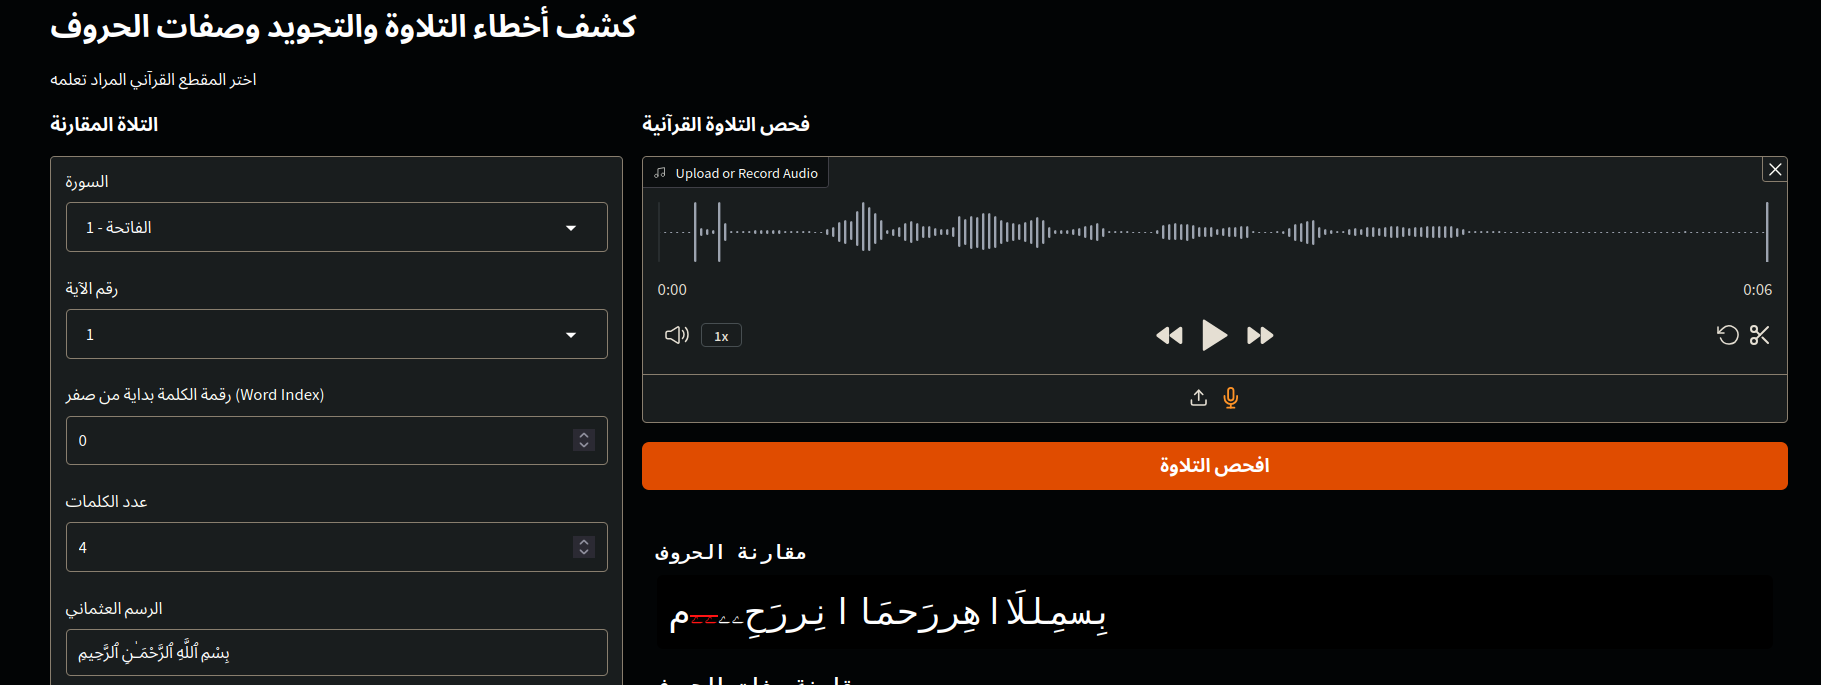
\includegraphics[width=0.8\textwidth]{../figures/gradio_ui_main.png}
\caption{Gradio Web App interface allowing users to test our model.}
\label{fig:gradio_main}
\end{figure}

\begin{figure}[H]
\centering
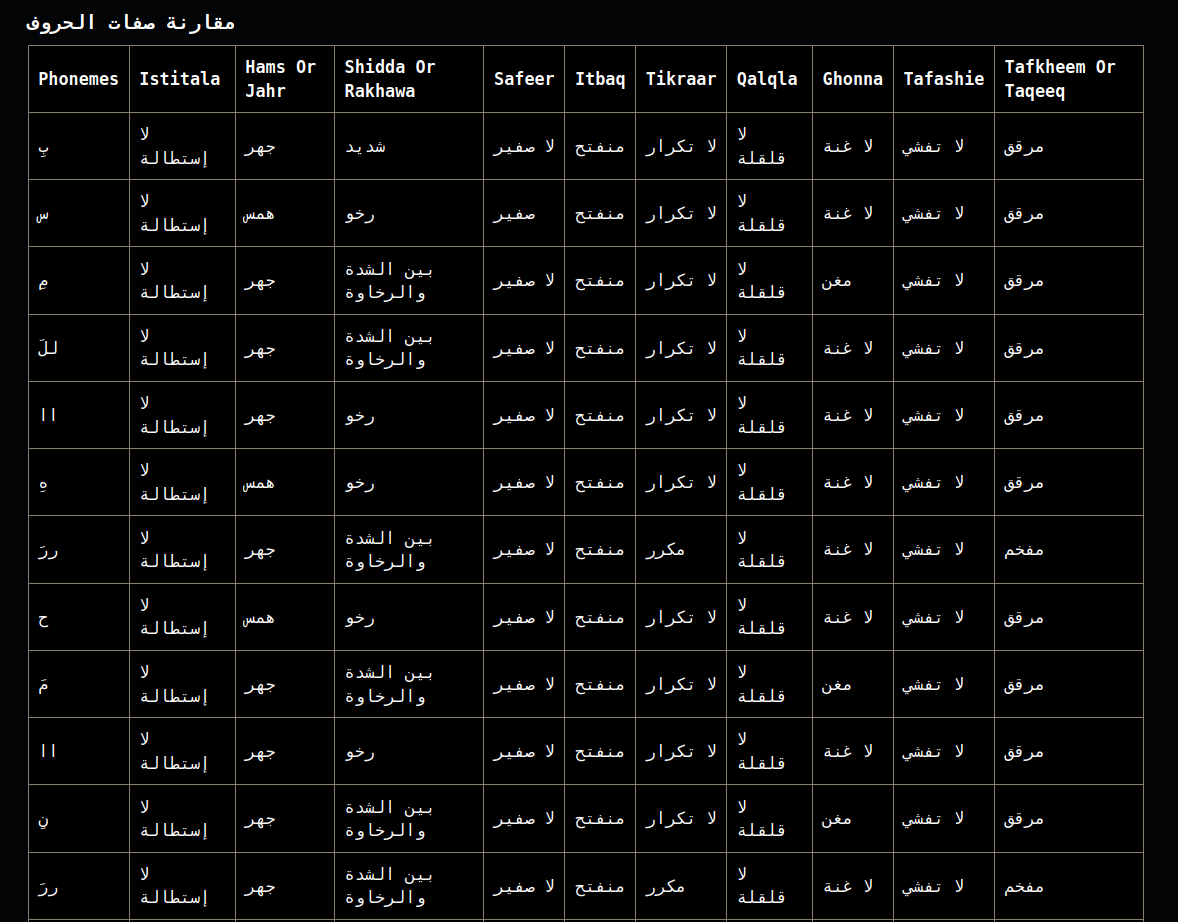
\includegraphics[width=0.8\textwidth]{../figures/gradio_ui_sifa.png}
\caption{Gradio Web App interface showing detailed Sifat (attribute) level feedback.}
\label{fig:gradio_sifa}
\end{figure}

User feedback has been extremely positive. Notably, the model generalized well to female voices despite being trained exclusively on male recitations, successfully detecting common errors such as incorrect \arb{مد} elongation or weak \arb{قلقلة} pronunciation. This demonstrates the robustness and practical applicability of our approach.



\section{Ablation Studies}

We conducted more than 13 experiments. To tune the weights for every level, we ran an evaluation set for each experiment on 20\% of the training data and logged the Phoneme Error Rate (PER) per level. Our goal was to minimize two metrics:
\begin{itemize}
\item Average Phoneme Error Rate (PER).
\item Standard deviation across all levels.
\end{itemize}

We report the best three experiments, labeled `EXP1`, `EXP2`, and `EXP3`. We adjusted the loss weight for every level in each experiment. The weight for the `phonemes` level was kept constant across all runs at 0.4, while the weights for `shidda_or_rakhawa` and `tafkheem_or_tarqeeq` were varied to achieve the best possible results.

\begin{longtable}{|l|c|c|c|}
\caption{The table above shows different loss weights applied to equation \ref{eq:multilevel_ctc} for three experiments: `EXP1`, `EXP2`, and `EXP3`. The `phonemes` level weight was kept constant across all runs. In each run, we tuned the weights for `shidda_or_rakhawa` and `tafkheem_or_tarqeeq` to minimize the average Phoneme Error Rate (PER) and the standard deviation across all levels. Note that the sum of all loss weights adds to 1.}
\label{tab:results_v2_weights}\\
\hline
\textbf{Attribute} & \textbf{EXP1} & \textbf{EXP2} & \textbf{EXP3} \\ 
\hline
\endfirsthead
\hline
\textbf{Attribute} & \textbf{EXP1} & \textbf{EXP2} & \textbf{EXP3} \\
\hline
\endhead
\hline
phonemes & 0.4 & 0.4 & 0.4 \\
\hline
tikraar & 0.06 & 0.058625 & 0.059625 \\
\hline
tafkheem_or_tarqeeq & 0.06 & 0.063 & 0.0060 \\
\hline
tafashie & 0.06 & 0.05825 & 0.059625 \\
\hline
Qalqala & 0.06 & 0.0585 & 0.059625 \\
\hline
Safeer & 0.06 & 0.05825 & 0.059625 \\
\hline
Shidda_or_rakhawa & 0.06 & 0.068 & 0.059625 \\
\hline
Istitala & 0.06 & 0.05825 & 0.059625 \\
\hline
Itbaaq & 0.06 & 0.05825 & 0.059625 \\
\hline
Ghonna & 0.060 & 0.05825 & 0.059625 \\
\hline
hams_or_jahr & 0.06 & 0.05825 & 0.059625 \\
\hline
average_per & 0.065 & 0.05825 & 0.059625 \\
\hline
std_per & 0.06 & 0.05825 & 0.059625 \\
\hline
\end{longtable}

We observed that `EXP3` yielded the best results, with an average PER of 0.293\% and a standard deviation of 0.0017, as shown in both Table \ref{tab:results_v2} and Figure \ref{fig:results_v2_std}. `EXP3` performed the best because it allocates more weight to levels that contain more labels—`shidda_or_rakhawa`—and to the more challenging level `tafkheem_or_tarqeeq`, without significantly affecting the rest of the levels.

\begin{figure}[H]
\centering
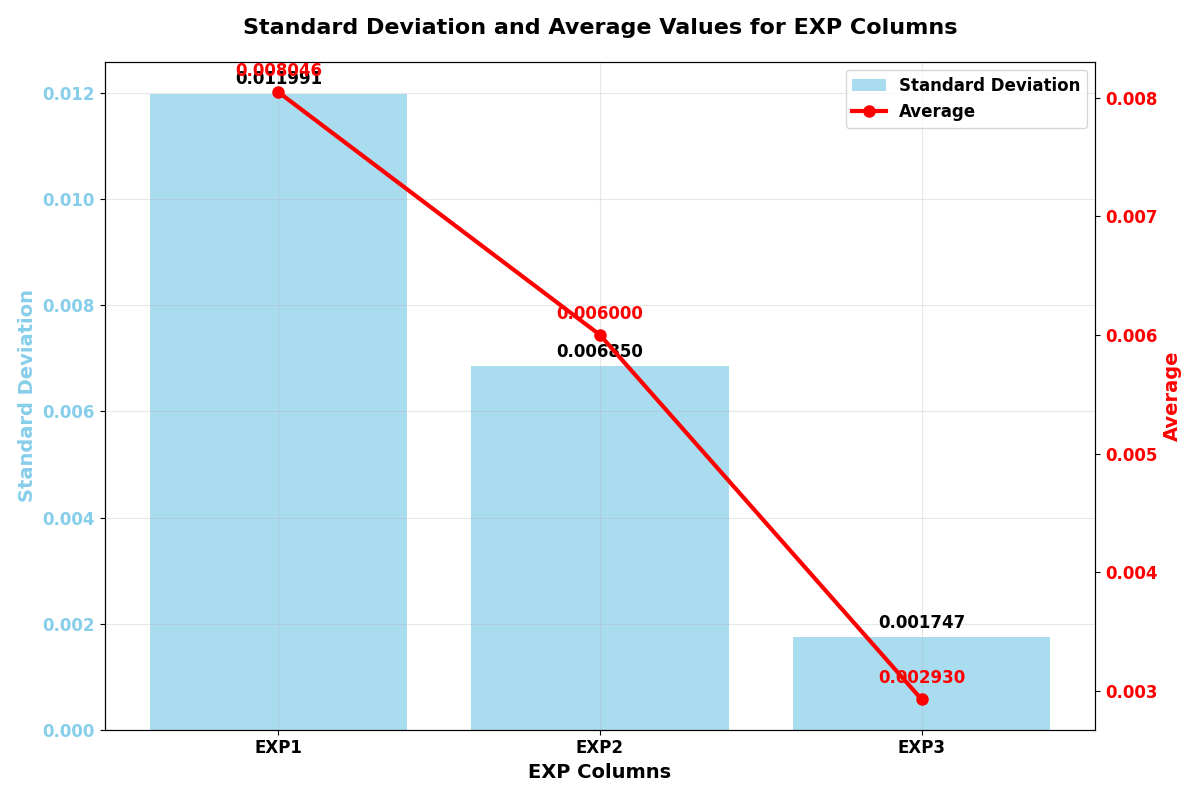
\includegraphics[width=0.8\textwidth]{./figures/results_stats_v2.png}
\caption{Average Phoneme Error Rate and Standard Deviation for all three runs. `EXP3` performs best by assigning higher weight to levels with more labels (`shidda_or_rakhawa`) and the more challenging `tafkheem_or_tarqeeq` level, without significant differences in the remaining levels.}
\label{fig:results_v2_std}
\end{figure}

\begin{longtable}{|l|c|c|c|}
\caption{Phoneme Error Rate for each level on 20\% of the training data. `EXP3` performs best by assigning higher weight to levels with more labels (`shidda_or_rakhawa`) and the more challenging `tafkheem_or_tarqeeq` level, without significant differences in the remaining levels.}
\label{tab:results_v2}\\
\hline
\textbf{Attribute} & \textbf{EXP1} & \textbf{EXP2} & \textbf{EXP3} \\ 
\hline
\endfirsthead
\hline
\textbf{Attribute} & \textbf{EXP1} & \textbf{EXP2} & \textbf{EXP3} \\
\hline
\endhead
\hline
phonemes & 0.0069 & 0.0069 & 0.0063 \\
\hline
tikraar & 0.006 & 0.006 & 0.0017 \\
\hline
tafkheem_or_tarqeeq & 0.002599 & 0.00279 & 0.0065 \\
\hline
tafashie & 0.001837 & 0.0025 & 0.0035 \\
\hline
Qalqala & 0.001808 & 0.008 & 0.00174 \\
\hline
Safeer & 0.00346 & 0.00246 & 0.00174 \\
\hline
Shidda_or_rakhawa & 0.015276 & 0.0053 & 0.0031 \\
\hline
Istitala & 0.00243 & 0.00166 & 0.001525 \\
\hline
Itbaaq & 0.00176 & 0.00217 & 0.00168 \\
\hline
Ghonna & 0.044 & 0.02675 & 0.00199 \\
\hline
hams_or_jahr & 0.0024 & 0.00256 & 0.00234 \\
\hline
average_per & 0.0080455 & 0.006 & 0.00293 \\
\hline
std_per & 0.0191 & 0.0062 & 0.0017 \\
\hline
\end{longtable}

After that we continued the training of `EXP3` that yields the results in \ref{tab:results}

\begin{figure}[H]
\centering
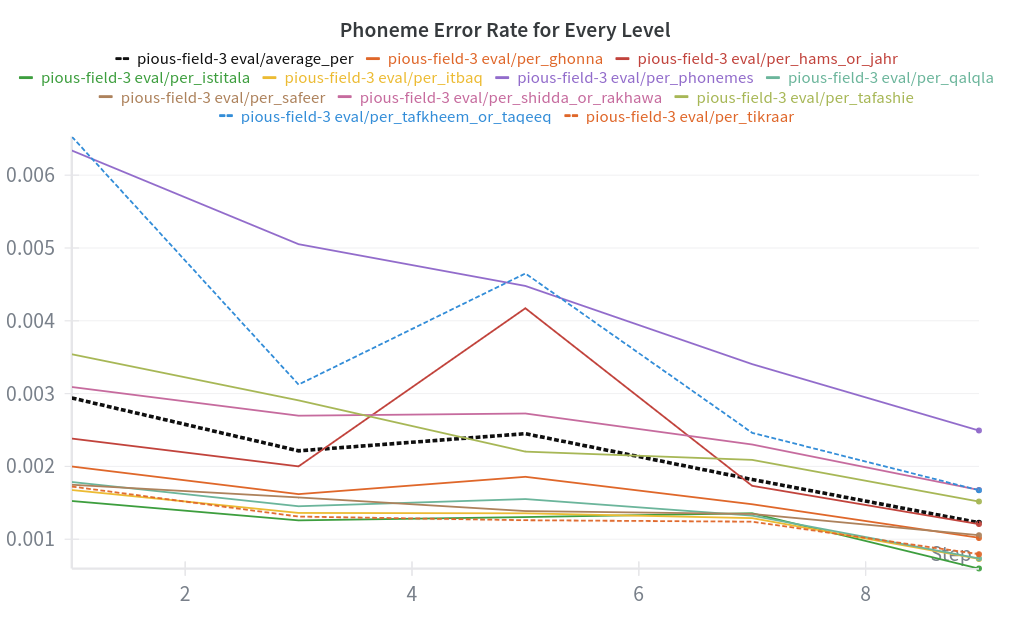
\includegraphics[width=\textwidth]{./figures/eval_v2_plot.png}
\caption{Evaluation PER during training steps}
\label{fig:eval_plot}
\end{figure}




% -------------------------------------------------------------
\section{Model Version 3}

After completing our initial training and publishing the model, we identified a minor bug and developed a new feature:

\begin{itemize}
\item \textbf{Bug Fix:} The model was incorrectly classifying a \arb{ياء} (\arb{ي}) with a \arb{شدة} as `yaa_madd` instead of as two separate \arb{ياء} characters.
\item \textbf{New Feature:} A third label, `low_mofakham`, was added to the `tafkheem_or_tarqeeq` level.
\end{itemize}

We trained this Version 3 model using the following loss weights: 0.4 for the `phonemes` level, 0.0605 for both `tafkheem_or_tarqeeq` and `shidda_or_rakhawa`, and 0.05987 for the remaining levels.

For testing, we removed \arb{مصاحف} `29.0` and `30.0` from the training and validation sets and combined them with the existing test set. This resulted in a final test set containing \arb{مصاحف} `19.0`, `26.1`, `29.0`, and `30.0`. The results are shown in Table \ref{tab:results_v3}.

\begin{longtable}{|l|c|}
\caption{Testing results on mosahaf `19.0`, `26.1`, `29.0`, and `30.0` showing a balanced Phoneme Error Rate (PER) across all levels. The `phonemes` level has a naturally higher PER as it is the largest vocabulary (44 tokens: 43 phonemes + 1 padding token).}
\label{tab:results_v3}\\
\hline
\textbf{Metric} & \textbf{Value} \\ 
\hline
\endfirsthead
\hline
\textbf{Metric} & \textbf{Value} \\
\hline
\endhead
per\_phonemes & 0.00449 \\
\hline
per\_hams\_or\_jahr & 0.00177 \\
\hline
per\_shidda\_or\_rakhawa & 0.00315 \\
\hline
per\_tafkheem\_or\_taqeeq & 0.00299 \\
\hline
per\_itbaq & 0.00130 \\
\hline
per\_safeer & 0.00152 \\
\hline
per\_qalqla & 0.00123 \\
\hline
per\_tikraar & 0.00436 \\
\hline
per\_tafashie & 0.00181 \\
\hline
per\_istitala & 0.00122 \\
\hline
per\_ghonna & 0.00185 \\
\hline
average\_per & 0.00234 \\
\hline
\end{longtable}
